\documentclass{article}
%\usepackage{geometry}
%\geometry{top = 1in, bottom = 1in, left = 1in, right = 1in}
\usepackage[top = 0.7in, bottom = 0.7in, left = 0.7in, right = 0.7in]{geometry}
\usepackage{amsmath,amssymb,amsthm,mathrsfs}
\usepackage{graphicx}
\usepackage{bm}
\usepackage{float}
\usepackage[font=footnotesize,labelfont=bf]{caption}
\usepackage{movie15}
\usepackage{hyperref}

\usepackage{fancyhdr}
\pagestyle{fancy}
\rhead{\footnotesize {MM/DD/2012 ; MESA version 4442} }
\chead{\footnotesize {Authors: Jared Brooks, Lars Bildsten, Bill Paxton} }
\lhead{\footnotesize {mesa/star/test\_suite/1M\_pre\_ms\_to\_wd} }

\begin{document}
	
	\begin{center}
	  \begin{Large}
	    \textbf{1M PRE MS TO WD}\\
	  \end{Large}
	\end{center}

        This test is to show a 1 $M_\odot$ pre-main sequence star evolved to a white dwarf.  Therefore, this test should be cut off when the log of the surface luminosity drops below -0.5 (\texttt{log\_L\_lower\_limit = -0.5}).\\

        The HR-diagram below shows the evolution through the whole run (figure \ref{fig:1}).

        \begin{figure}[H]
          \centering
          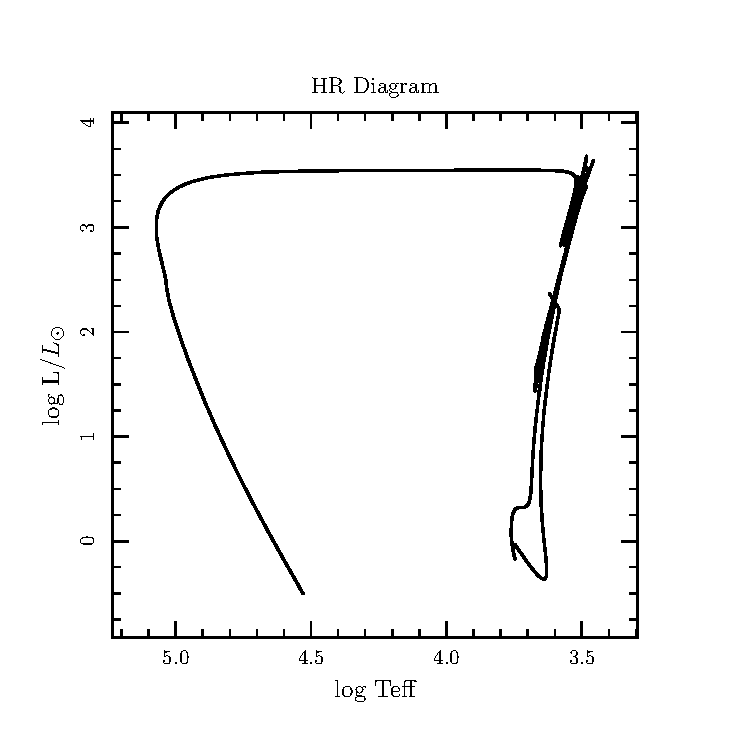
\includegraphics[width = 5in]{/Users/jaredbrooks/1M_pre_ms_to_wd/plots_out/HR_Diagram.pdf}
          \caption{HR-diagram showing pre-MS, MS, RGB, AGB, and WD phases}
          \label{fig:1}
        \end{figure}

        \pagebreak

        To the left is an HR-diagram showing the pre-MS and the main sequence (figure \ref{fig:2}).  To the right is a temperature-density profile from the main sequence (figure \ref{fig:3}).

        \begin{figure}[H]
          \begin{minipage}[b]{0.5\linewidth}
            \centering
            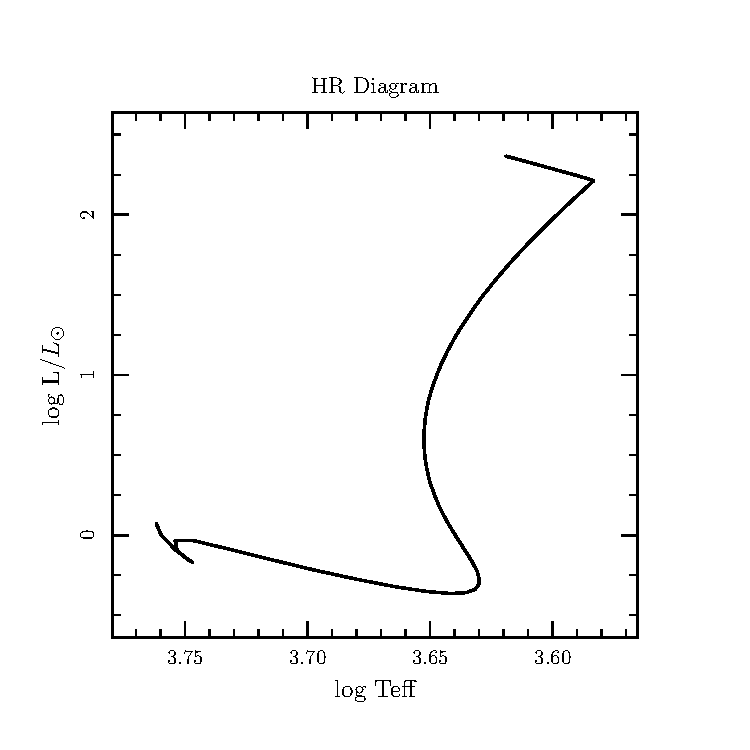
\includegraphics[width = 3.8in]{/Users/jaredbrooks/1M_pre_ms_to_wd/plots_out/HR_Diagram_MS.pdf}
            \caption{HR-diagram of pre-MS and MS}
            \label{fig:2}
          \end{minipage}
          \hspace{0cm}
          \begin{minipage}[b]{0.5\linewidth}
            \centering
            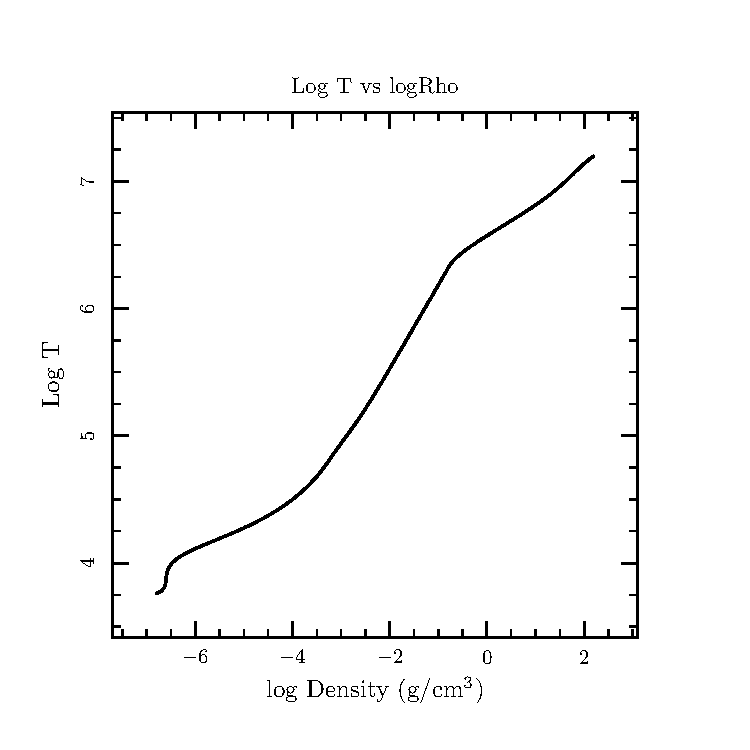
\includegraphics[width = 3.8in]{/Users/jaredbrooks/1M_pre_ms_to_wd/plots_out/Log_T_vs_logRho_18.pdf}
            \caption{Temperature density profile from MS}
            \label{fig:3}
          \end{minipage}
        \end{figure}

        Below are an abundance profile (figure \ref{fig:4}) and a burning rate profile (figure \ref{fig:5}) from the main sequence.

        \begin{figure}[H]
          \begin{minipage}[b]{0.5\linewidth}
	    \centering
	    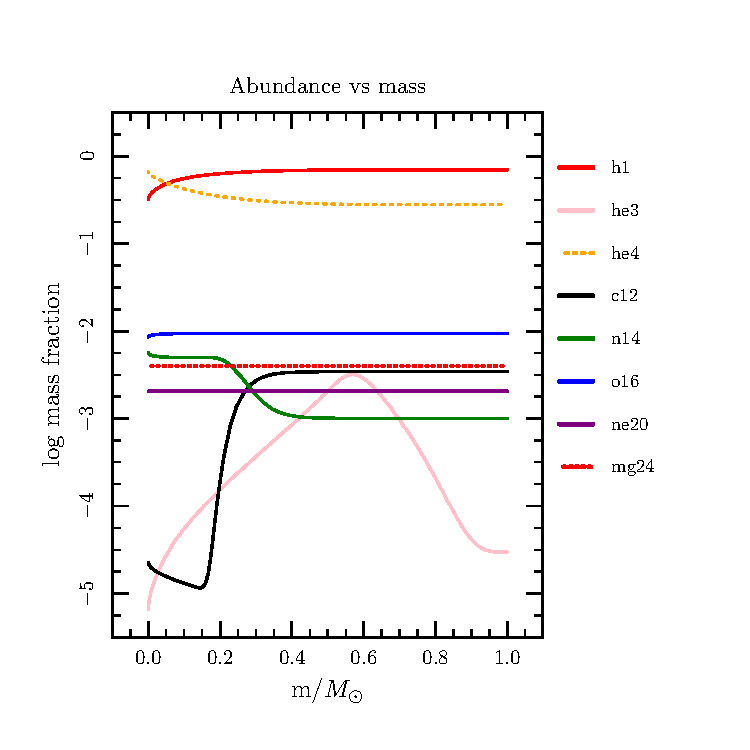
\includegraphics[width = 3.8in]{/Users/jaredbrooks/1M_pre_ms_to_wd/plots_out/Abundance_vs_mass_18.pdf}
	    \caption{Abundance profile at MS}
	    \label{fig:4}
          \end{minipage}
          \hspace{0cm}
          \begin{minipage}[b]{0.5\linewidth}
            \centering
            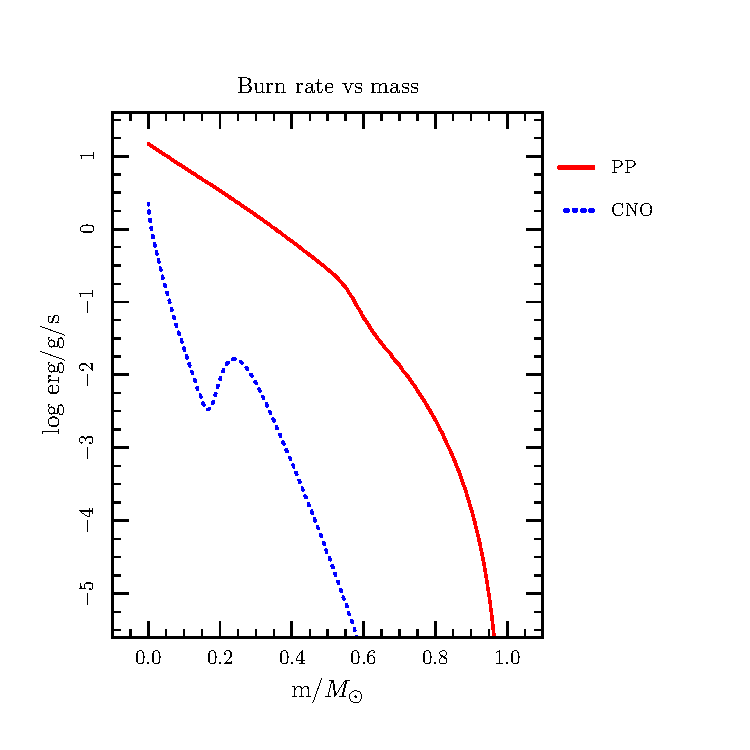
\includegraphics[width = 3.8in]{/Users/jaredbrooks/1M_pre_ms_to_wd/plots_out/Burnrate_vs_mass_18.pdf}
            \caption{Burning rate profile at MS}
            \label{fig:5}
          \end{minipage}
	\end{figure}

        \pagebreak

        To the left is an HR-diagram showing the end of the main sequence and the RGB, with the helium core flash in the upper right corner (figure \ref{fig:6}).  To the right is a temperature-density profile from the RGB (figure \ref{fig:7}).

        \begin{figure}[H]
          \begin{minipage}[b]{0.5\linewidth}
            \centering
            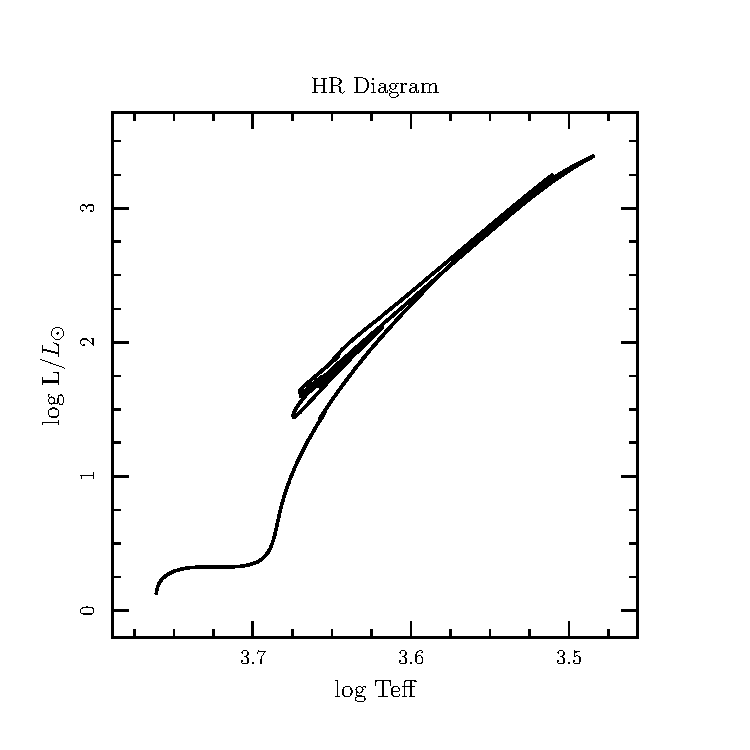
\includegraphics[width = 3.8in]{/Users/jaredbrooks/1M_pre_ms_to_wd/plots_out/HR_Diagram_RGB.pdf}
            \caption{HR-diagram of RGB}
            \label{fig:6}
          \end{minipage}
          \hspace{0cm}
          \begin{minipage}[b]{0.5\linewidth}
            \centering
            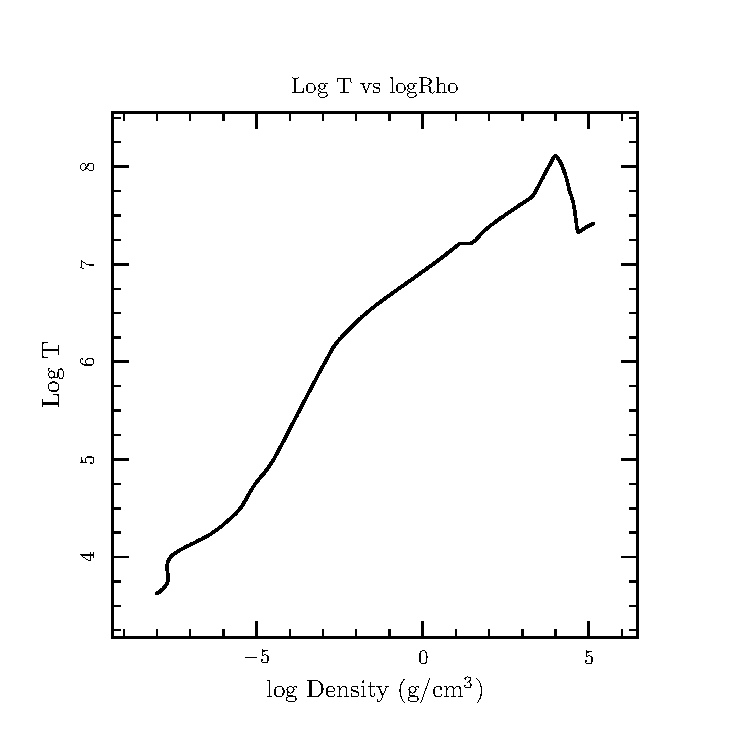
\includegraphics[width = 3.8in]{/Users/jaredbrooks/1M_pre_ms_to_wd/plots_out/Log_T_vs_logRho_36.pdf}
            \caption{Temperature density profile from RGB}
            \label{fig:7}
          \end{minipage}
        \end{figure}

        Below are an abundance profile (figure \ref{fig:8}) and a burning rate profile (figure \ref{fig:9}) from the RGB.

        \begin{figure}[H]
          \begin{minipage}[b]{0.5\linewidth}
	    \centering
	    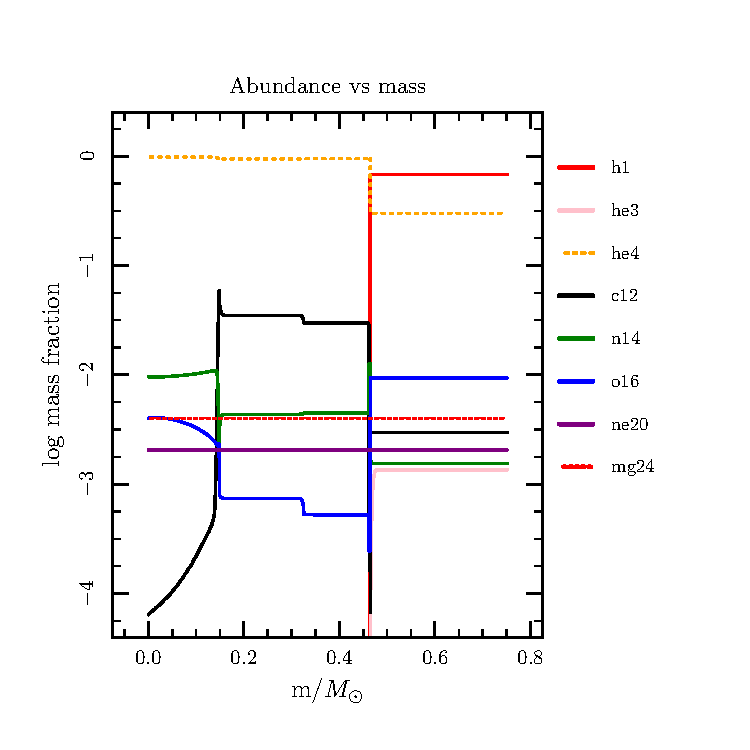
\includegraphics[width = 3.8in]{/Users/jaredbrooks/1M_pre_ms_to_wd/plots_out/Abundance_vs_mass_36.pdf}
	    \caption{Abundance profile at RGB}
	    \label{fig:8}
          \end{minipage}
          \hspace{0cm}
          \begin{minipage}[b]{0.5\linewidth}
            \centering
            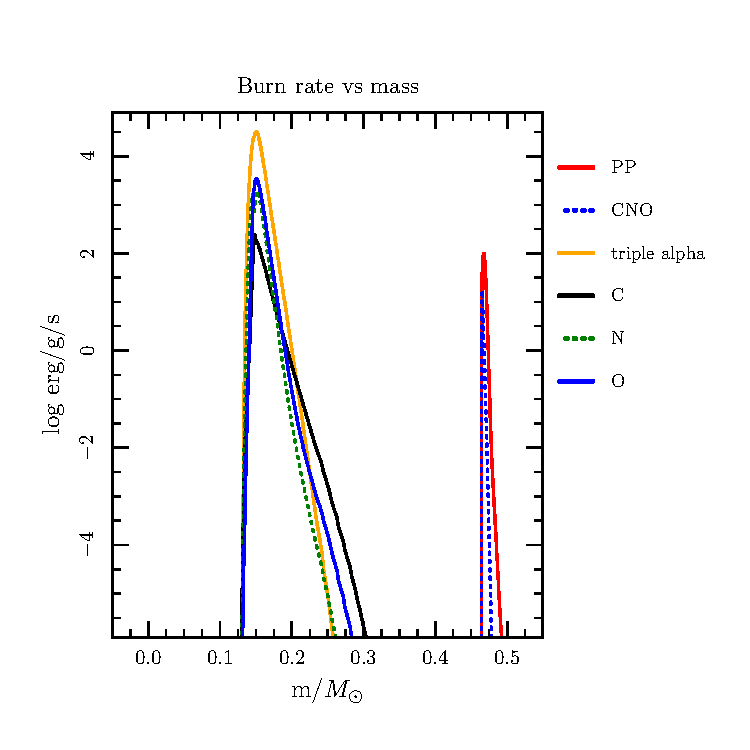
\includegraphics[width = 3.8in]{/Users/jaredbrooks/1M_pre_ms_to_wd/plots_out/Burnrate_vs_mass_36.pdf}
            \caption{Burning rate profile at RGB}
            \label{fig:9}
          \end{minipage}
	\end{figure}

        \pagebreak

        To the left is an HR-diagram showing the early AGB (figure \ref{fig:10}).  To the right is a temperature-density profile from the early AGB (figure \ref{fig:11}).

        \begin{figure}[H]
          \begin{minipage}[b]{0.5\linewidth}
            \centering
            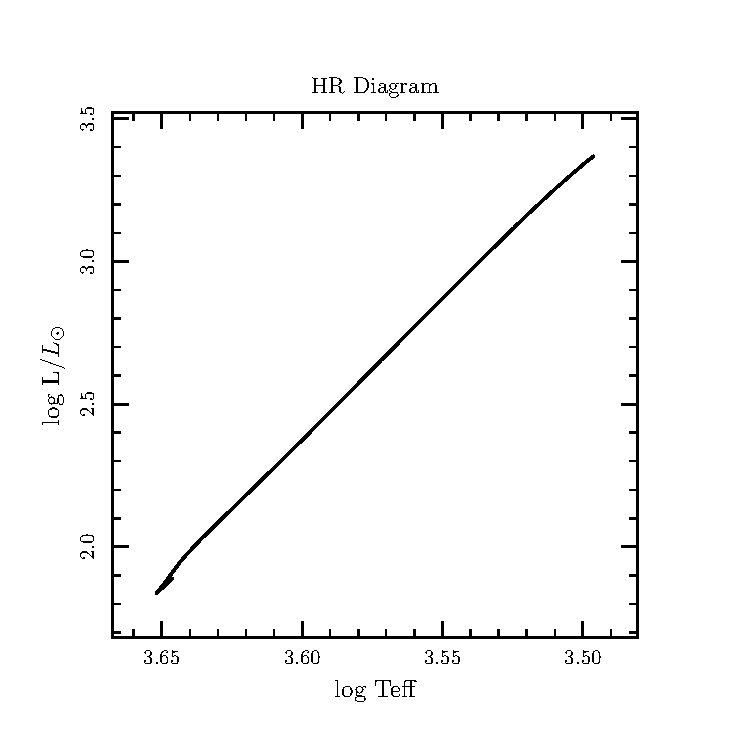
\includegraphics[width = 3.8in]{/Users/jaredbrooks/1M_pre_ms_to_wd/plots_out/HR_Diagram_E_AGB.pdf}
            \caption{HR-diagram of early AGB}
            \label{fig:10}
          \end{minipage}
          \hspace{0cm}
          \begin{minipage}[b]{0.5\linewidth}
            \centering
            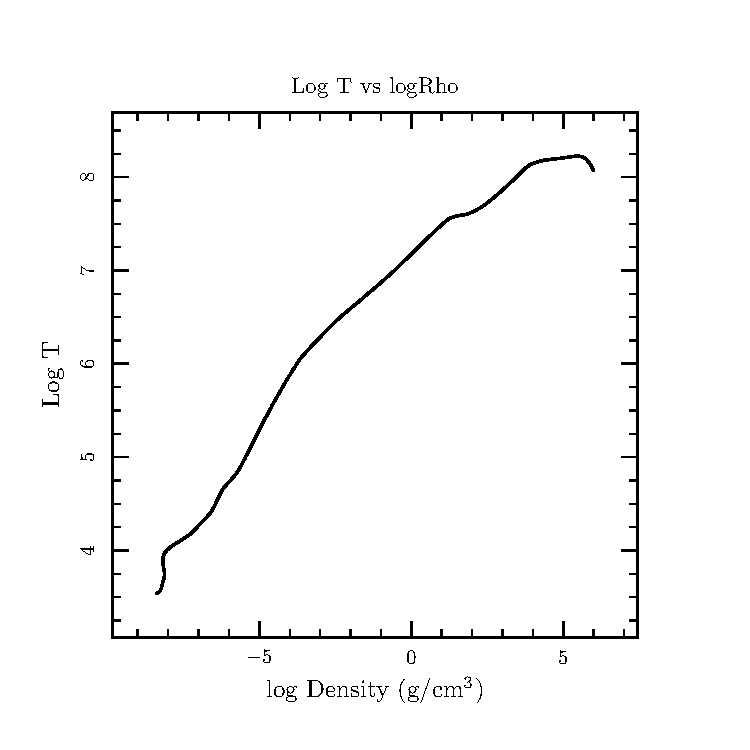
\includegraphics[width = 3.8in]{/Users/jaredbrooks/1M_pre_ms_to_wd/plots_out/Log_T_vs_logRho_76.pdf}
            \caption{Temperature density profile from early AGB}
            \label{fig:11}
          \end{minipage}
        \end{figure}

        Below are an abundance profile (figure \ref{fig:12}) and a burning rate profile (figure \ref{fig:13}) from the early AGB.

        \begin{figure}[H]
          \begin{minipage}[b]{0.5\linewidth}
            \centering
            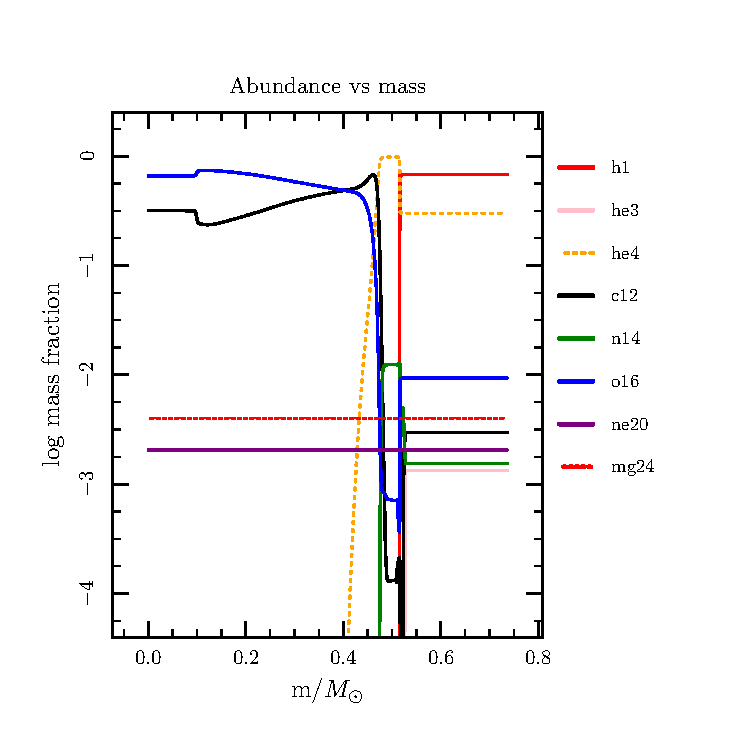
\includegraphics[width = 3.8in]{/Users/jaredbrooks/1M_pre_ms_to_wd/plots_out/Abundance_vs_mass_76.pdf}
            \caption{Abundance profile at early AGB}
            \label{fig:12}
          \end{minipage}
          \hspace{0cm}
          \begin{minipage}[b]{0.5\linewidth}
            \centering
            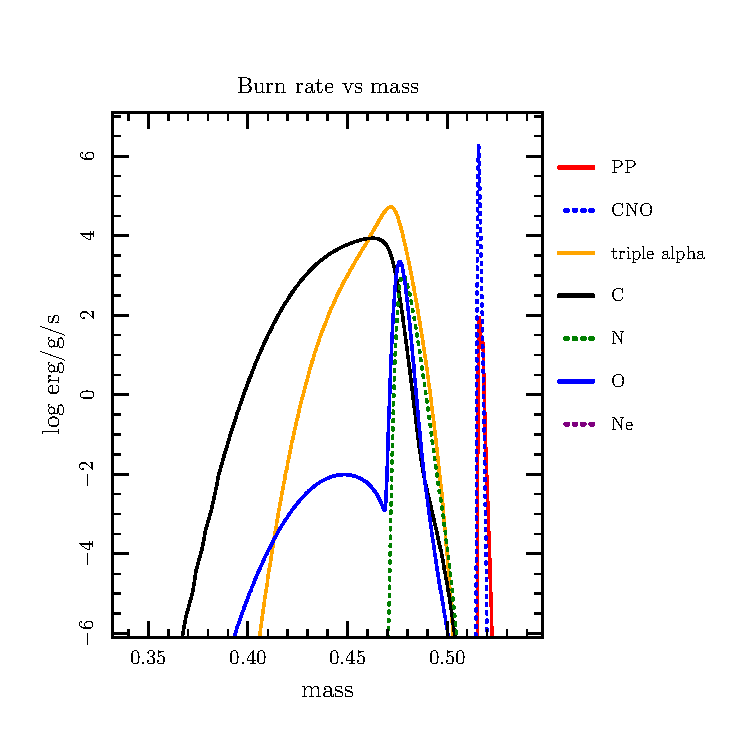
\includegraphics[width = 3.8in]{/Users/jaredbrooks/1M_pre_ms_to_wd/plots_out/Burnrate_vs_mass_76.pdf}
            \caption{Burning rate profile at early AGB}
            \label{fig:13}
          \end{minipage}
        \end{figure}

        \pagebreak

        To the left is an HR-diagram showing the thermally pulsing AGB (figure \ref{fig:14}).  To the right is a temperature-density profile from the thermally pulsing AGB (figure \ref{fig:15}).

        \begin{figure}[H]
          \begin{minipage}[b]{0.5\linewidth}
            \centering
            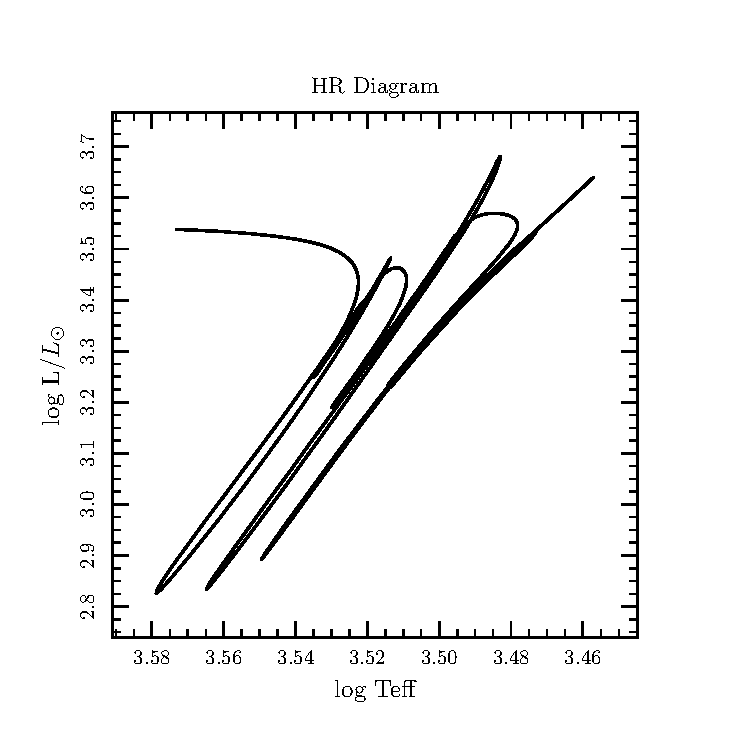
\includegraphics[width = 3.8in]{/Users/jaredbrooks/1M_pre_ms_to_wd/plots_out/HR_Diagram_TP_AGB.pdf}
            \caption{HR-diagram of thermally pulsing AGB}
            \label{fig:14}
          \end{minipage}
          \hspace{0cm}
          \begin{minipage}[b]{0.5\linewidth}
            \centering
            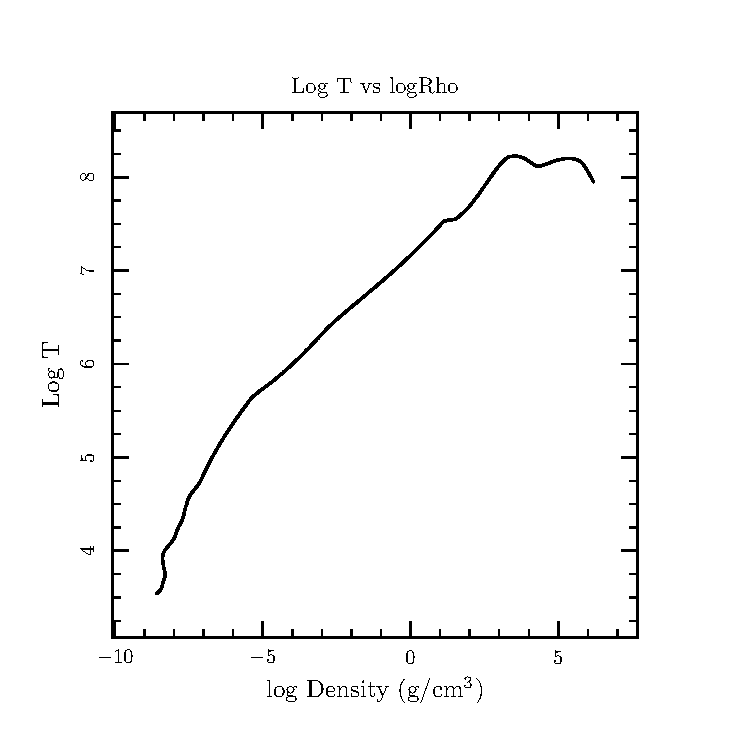
\includegraphics[width = 3.8in]{/Users/jaredbrooks/1M_pre_ms_to_wd/plots_out/Log_T_vs_logRho_41.pdf}
            \caption{Temperature density profile from thermally pulsing AGB}
            \label{fig:15}
          \end{minipage}
        \end{figure}

        Below are two burning rate profiles from the thermally pulsing AGB phase.  The one on the left (figure \ref{fig:16}) shows dominant helium burning during one of the pulses.  The one on the right (figure \ref{fig:17}) shows dominant hydrogen burning between pulses.

        \begin{figure}[H]
          \begin{minipage}[b]{0.5\linewidth}
            \centering
            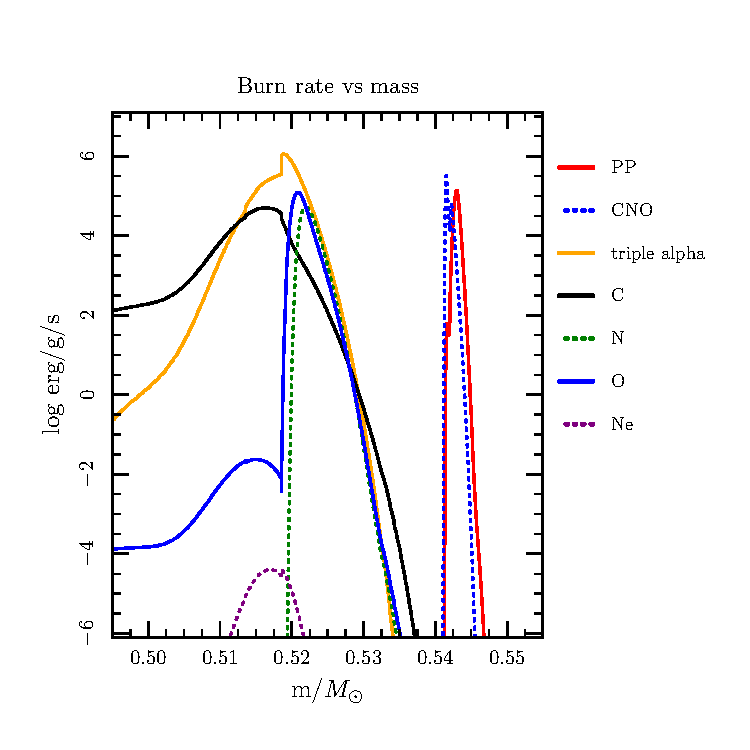
\includegraphics[width = 3.8in]{/Users/jaredbrooks/1M_pre_ms_to_wd/plots_out/Burnrate_vs_mass_41.pdf}
            \caption{Burning rate profile during thermal pulse}
            \label{fig:16}
          \end{minipage}
          \hspace{0cm}
          \begin{minipage}[b]{0.5\linewidth}
            \centering
            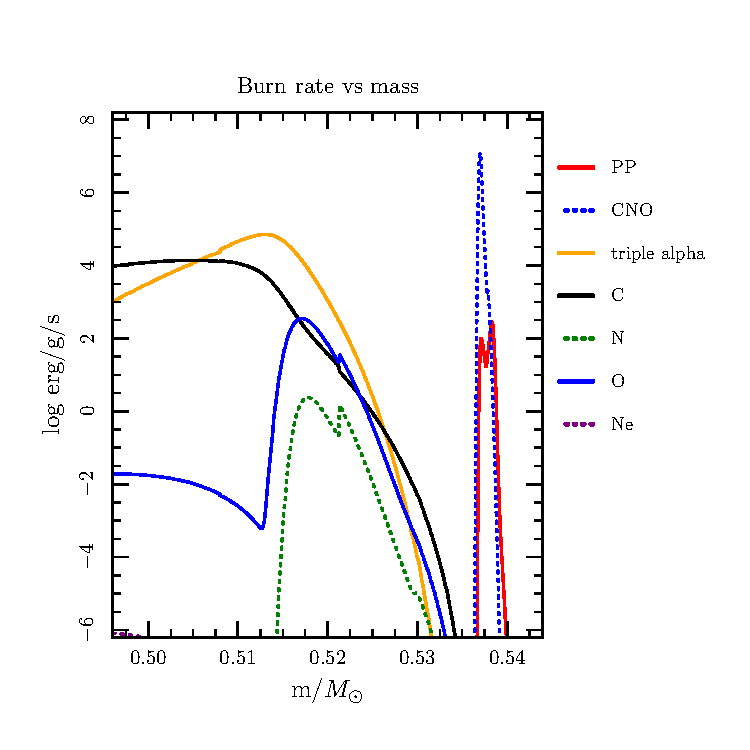
\includegraphics[width = 3.8in]{/Users/jaredbrooks/1M_pre_ms_to_wd/plots_out/Burnrate_vs_mass_58.pdf}
            \caption{Burning rate profile between pulses}
            \label{fig:17}
          \end{minipage}
        \end{figure}

        \pagebreak

        To the left is an HR-diagram showing the transition from AGB to white dwarf (figure \ref{fig:18}).  To the right is a temperature-density profile from the end of the run (figure \ref{fig:19}).

        \begin{figure}[H]
          \begin{minipage}[b]{0.5\linewidth}
            \centering
            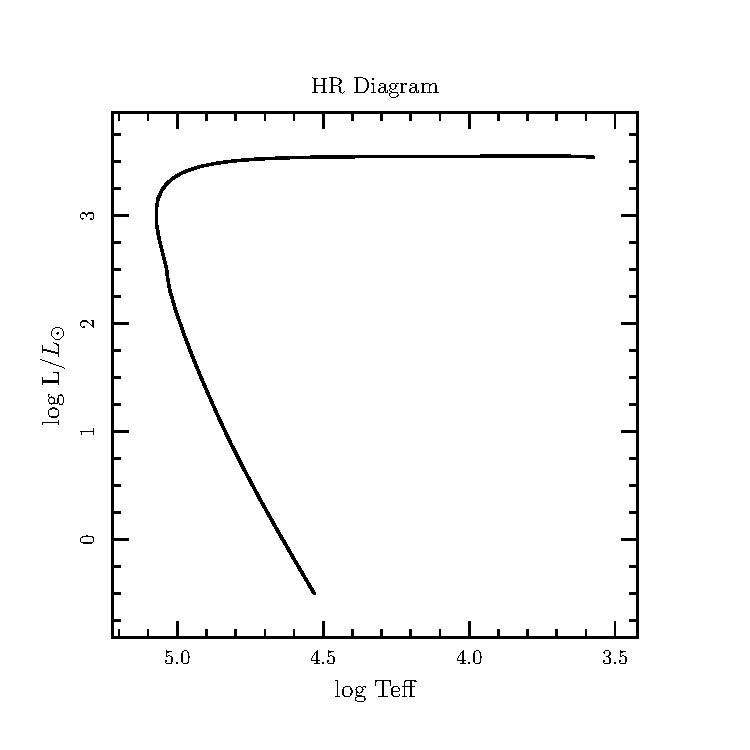
\includegraphics[width = 3.8in]{/Users/jaredbrooks/1M_pre_ms_to_wd/plots_out/HR_Diagram_WD.pdf}
            \caption{HR-diagram shows AGB to WD}
            \label{fig:18}
          \end{minipage}
          \hspace{0cm}
          \begin{minipage}[b]{0.5\linewidth}
            \centering
            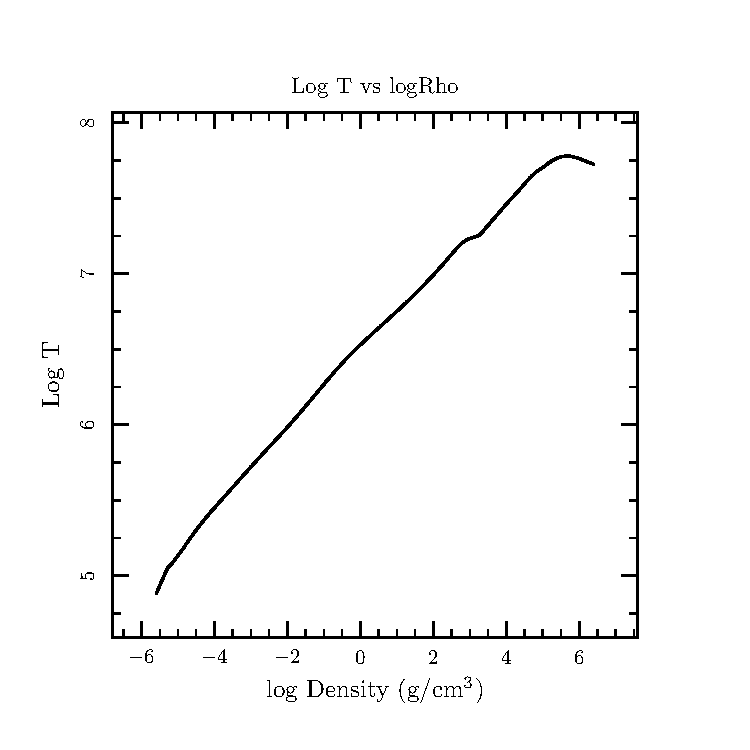
\includegraphics[width = 3.8in]{/Users/jaredbrooks/1M_pre_ms_to_wd/plots_out/Log_T_vs_logRho_43.pdf}
            \caption{Temperature density profile from end of run}
            \label{fig:19}
          \end{minipage}
        \end{figure}

        To the left in an abundance profile from the end of the run (figure \ref{fig:20}), plotted against logxq where logxq = log(1-q) and q is the fraction of star mass interior to outer boundary of each zone, moving outward from the core.  To the right is plot of the evolution of the center temperature and density for the entire run (figure \ref{fig:21}).

        \begin{figure}[H]
          \begin{minipage}[b]{0.5\linewidth}
            \centering
            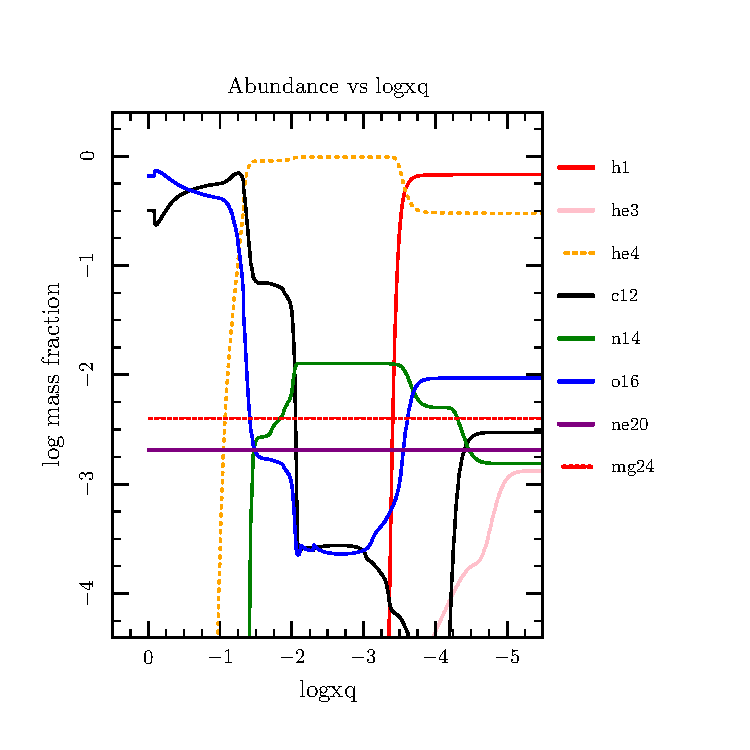
\includegraphics[width = 3.8in]{/Users/jaredbrooks/1M_pre_ms_to_wd/plots_out/Abundance_vs_logxq_43.pdf}
            \caption{Abundance profile from end of run}
            \label{fig:20}
          \end{minipage}
          \hspace{0cm}
          \begin{minipage}[b]{0.5\linewidth}
            \centering
            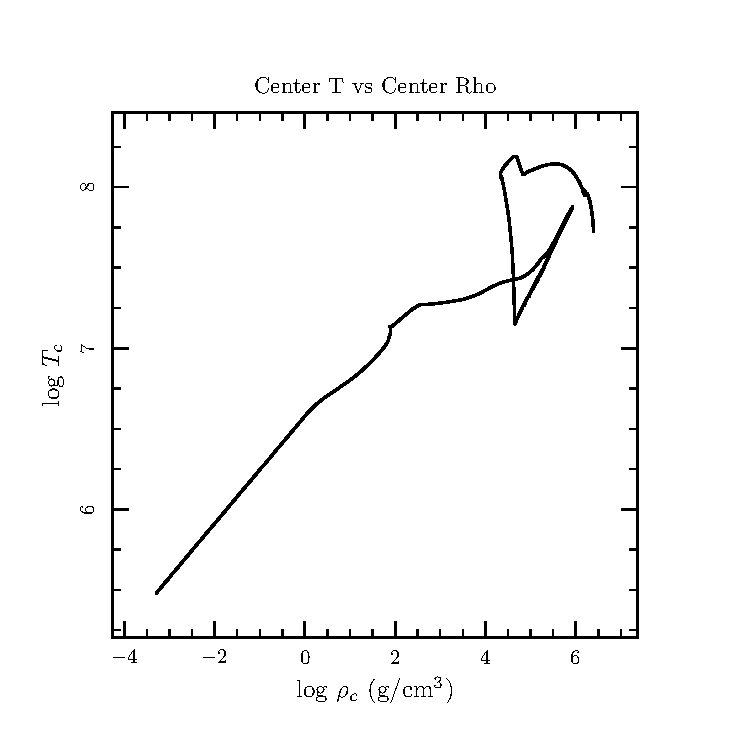
\includegraphics[width = 3.8in]{/Users/jaredbrooks/1M_pre_ms_to_wd/plots_out/Tc_vs_Rhoc.pdf}
            \caption{Evolution of center temperature and density}
            \label{fig:21}
          \end{minipage}
        \end{figure}

        \pagebreak

        This final plot (figure \ref{fig:22}) shows a few internal \texttt{MESA} variables, such as the size of the time-step, the number of zones, and the number of retries against the model number in order to give some understanding of how hard \texttt{MESA} is working throughout the run and where some areas of problems/interest might be.

        \begin{figure}[H]
          \centering
          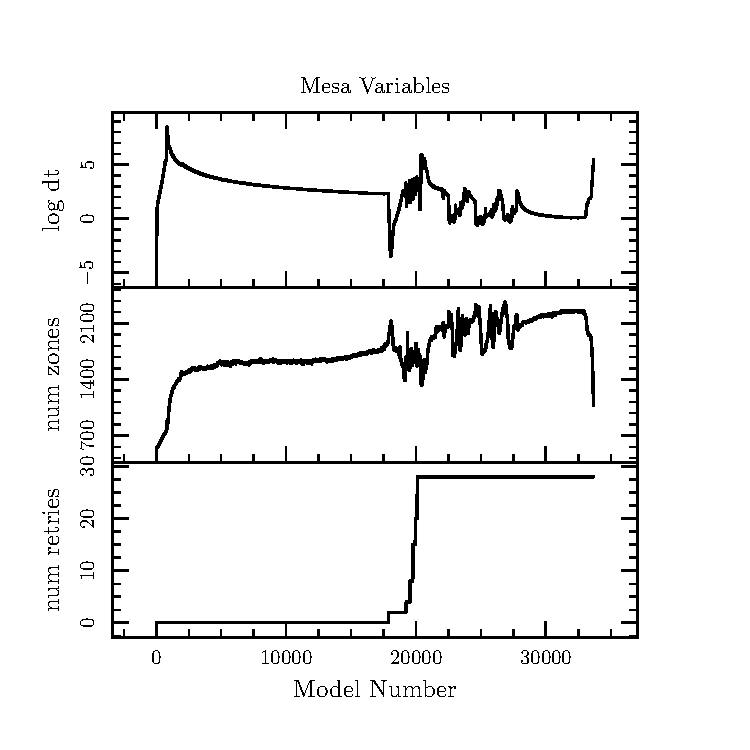
\includegraphics[width = 5in]{/Users/jaredbrooks/1M_pre_ms_to_wd/plots_out/Mesa_Variables.pdf}
          \caption{\texttt{MESA} variables plotted against model number show how hard \texttt{MESA} is working}
          \label{fig:22}
        \end{figure}


\end{document}
